\documentclass{resume}

\begin{document}

\fontfamily{ppl}\selectfont

\noindent
\begin{tabularx}{\linewidth}{@{}m{0.8\textwidth} m{0.2\textwidth}@{}}
{
    \Large{Emanuel Moraes de Almeida} \newline
    \small{
        \clink{
            \href{mailto:emanuelmoraes297@gmail.com}{emanuelmoraes297@gmail.com} $\cdot$ 
            {\fontdimen2\font=0.75ex +55 88 99287 8885}
            \href{https://github.com/emanuelmoraes-dev}{https://github.com/emanuelmoraes-dev}
            
            \href{https://www.linkedin.com/in/emanuel-moraes-de-almeida-346055187}{https://www.linkedin.com/in/emanuel-moraes-de-almeida-346055187}
        } \newline
        Ceará, BRASIL
    }
} & 
{
    \hfill
    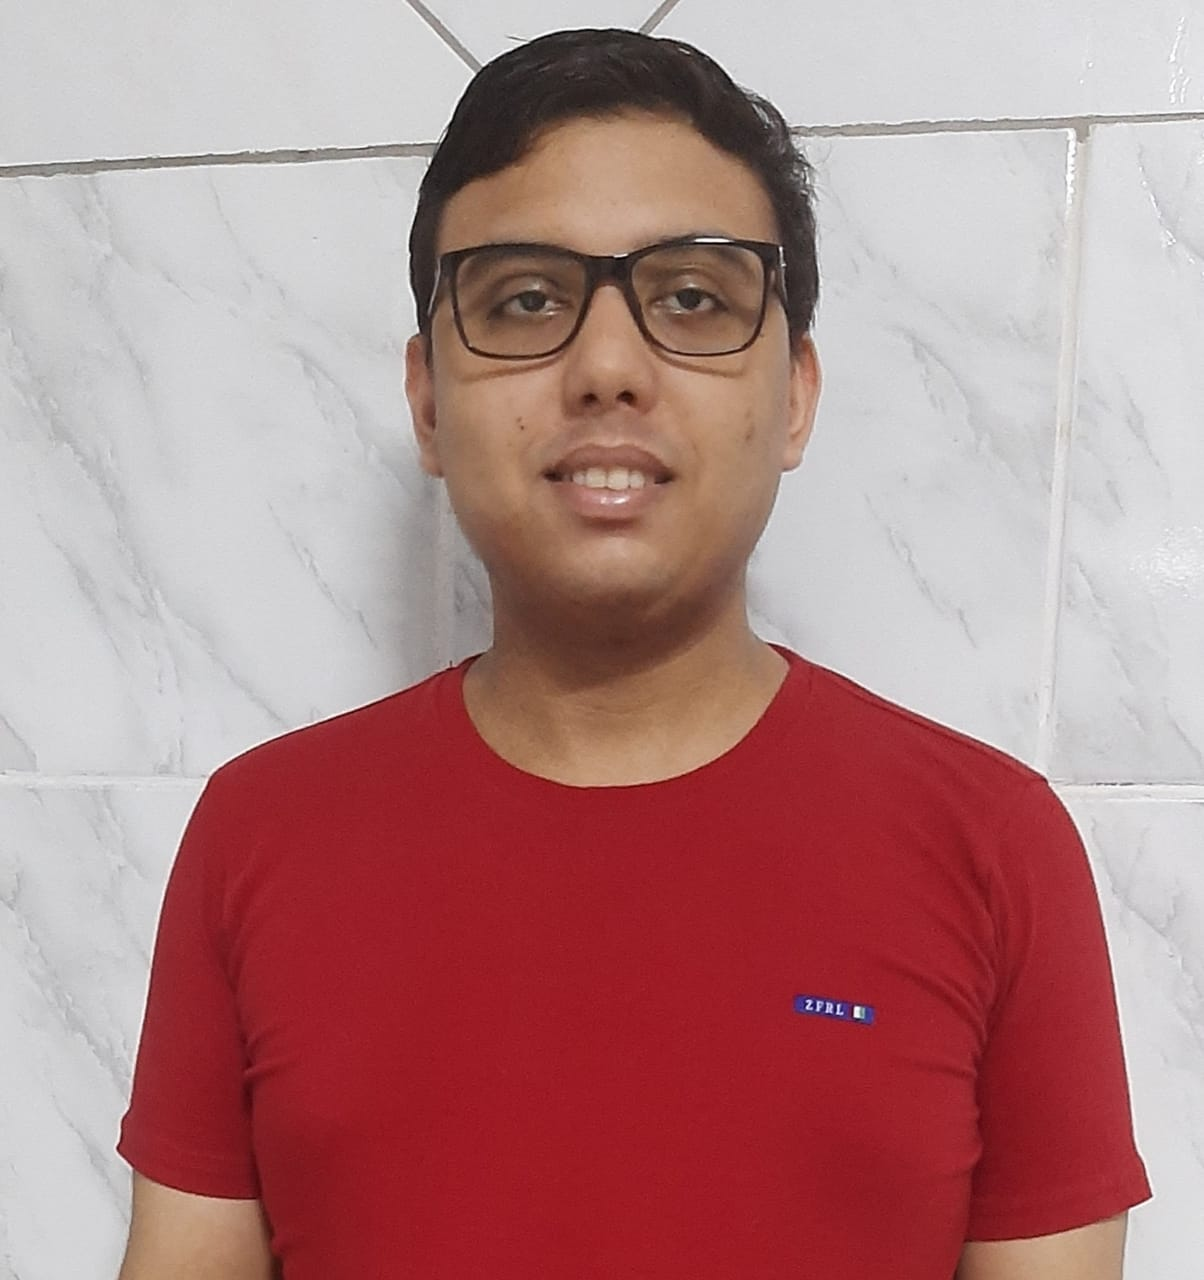
\includegraphics[width=2.8cm]{images/face.jpeg}
}
\end{tabularx}

\begin{center}
\begin{tabularx}{\linewidth}{@{}*{2}{X}@{}}
% left side %
{
    \csection{EDUCAÇÃO}{\small
        \begin{itemize}
            \item \frcontent{Bacharel em Ciência da Computação}{Instituto Federal de Educação, Ciência e Tecnologia do Ceará (IFCE), Campus Aracati, BRASIL}{}{2015-2020}
            
            \item \frcontent{Curso técnico/profissionalizante em Técnico em Informática}{Instituto Federal de Educação, Ciência e Tecnologia do Ceará (IFCE), Campus Aracati, BRASIL}{}{2014-2015}
        \end{itemize}
    }
    \csection{EXPERIÊNCIA}{\small
        \begin{itemize}
            \item \frcontent{Laboratório de Redes e Sistemas (LAR) - IFCE}{Bolsista - IFCE - Aracati.}{Desenvolvedor backend do BENTHAM, uma plataforma inteligente de controle e planejamento de programas e projetos de obras civil.}{2017-2020}
            
            \item \frcontent{Maratona de Programação}{Bolsista - IFCE - Aracati.}{Bolsa de pesquisa sobre Teoria da Computação e Estrutura de Dados para preparação para a Maratona de Programação e a Olimpíada Brasileira de Informática (OBI).}{2015}
            
            \item \frcontent{\href{https://launchertech.com/}{Launcher Tech}}{Desenvolvedor Full Stack.}{Desenvolvimento frontend (VueJS) e backend (NodeJS), tanto para disponibilizar páginas WEB, quanto para a disponibilização de funcionalidades mais dinâmicas, como autenticação, cadastros, buscas, internacionalização, entre outros. Também foram desenvolvidas algumas APIs e frameworks para automatizar o desenvolvimento de alguns tipos de aplicações frontend e backend (VueJS e PHP).}{2016, 2018-atualmente}
        \end{itemize}
    }
} 
% end left side %
& 
% right side %
{
    \csection{HABILIDADES}{\small
        \begin{itemize}
            \item \textbf{Linguagens} \newline
            {\footnotesize JavaScript, TypeScript, C, C++, Java, Python, PHP, SQL, Shell Script.}{}{}
        
            \item \textbf{Tecnologias} \newline
            {\footnotesize NodeJS, ExpressJS, Webpack, VueJS, ElectronJS, Spring (java), Flask (python), Lumen (PHP), Docker, MongoDB, Hibernate, TypeORM.}{}{}

            \item \textbf{Padrões \& Práticas} \newline
            {\footnotesize Programação Orientada a Objetos, Programação Funcional e Programação Reativa.}
        \end{itemize}
    }
    \csection{PRÊMIOS \& RECONHECIMENTO}{\small
        \begin{itemize}
            \item \frcontent{Olimpíada Brasileira de Informática (OBI)}{Premiado em 11ª colocação (medalha de bronze), na modalidade universitária.}{}{2015}
        \end{itemize}
    }
    \csection{LÍNGUAS}{\small
        \begin{itemize}
        
            \item Português (Língua materna)
            \item Inglês (Básico)
        \end{itemize}
    }
    \csection{PROJETOS}{\small
        \begin{itemize}
            \item \frcontent{Bentham}{Uma plataforma inteligente de controle e planejamento de programas e projetos de obras civil. Foi desenvolvido no Laboratório de Redes e Sistemas do IFCE, Campus Aracati, em parceria com a \href{https://www.quantaconsultoria.com/}{Quanta}, fomentado pela \href{https://embrapii.org.br/}{EMBRAPII}.\newline
            \textbf{INPI:} BR512019000592-9
            }{\textbf{Backend:} Java, Spring, JasperReports, Hibernate, PostgreSQL.}{2017-2020}
        \end{itemize}
    }
}
\end{tabularx}
\end{center}

\newpage

\begin{center}
\begin{tabularx}{\linewidth}{@{}*{2}{X}@{}}
% left side %
{
    \csection{PROJETOS}{\small
        \begin{itemize}
            \item \frcontent{\href{https://www.npmjs.com/package/alpha-restful}{Alpha Restful}}{Um framework para o desenvolvimento de aplicações WEB REST Backend em NodeJS, feito para MongoDB. Este framework é uma prova de conceito que busca mudar a maneira como as entidades são modeladas no MongoDB. Em conjunto com a ORM Mongoose, o Alpha Restful apresenta-se como uma camada de abstração para facilitar a implementação de diversas funcionalidades sobre dados que precisem ser normalizados no MongoDB. Mais informações podem ser obtidas através do meu \href{https://github.com/emanuelmoraes-dev/TCC-II/blob/main/documento.pdf}{Trabalho de Conclusão de Curso (TCC)}. Apesar de ser apenas uma prova de conceito em fase beta, a sua  \href{https://www.npmjs.com/package/alpha-restful}{página inicial no NPM} registra vários downloads semanais.}{\textbf{Backend:} JavaScript, NodeJS, MongoDB, MongooseJS.}{2019-2020}
            
            \item \frcontent{Manager}{O Manager consiste em um conjunto de APIs e frameworks capazes de automatizar o desenvolvimento de gerenciadores para sites, bem como a parte do backend (em Lumen (PHP)). O Manager é capaz de, automaticamente, gerar um frontend (gerenciador) que altera os textos e adiciona imagens e vídeos em outros sites que foram desenvolvidos usando um padrão pré-estabelecido. As rotas em PHP são geradas automaticamente e com poucas linhas, um sistema gerenciador é criado, na qual o cliente poderá alterar os textos de seu próprio site ou alterar as mídias ali apresentes. O Manager é um projeto de código privado e ainda está em fase de desenvolvimento, por meio da Launcher Tech.}{\textbf{FullStack:} VueJS, PHP, Lumen.}{2020-atualmente}
            
            \item \frcontent{Auto Acadêmico}{Um sistema desenvolvido por meio da Launcher Tech para que os alunos possam interagir, através de uma aplicação Android, com a auto escola. A ideia é que o aluno apenas precise sair de sua casa para realizar a aula, e todo o resto possa ser feito de forma virtual, inclusive a escolha de quais alunos entrariam em quais aulas ou eventos. O sistema foi 100\% finalizado e é completamente funcional. Apesar disso ele não pôde entrar em produção, graças a aplicações que posteriormente foram disponibilizadas de maneira oficial pelo governo.}{\textbf{FullStack:} VueJS, Express (NodeJS).}{2018-2019}
        \end{itemize}
    }
} 
% end left side %
& 
% right side %
{
    \csection{}{\small
        \begin{itemize}
            \item \frcontent{\href{https://www.npmjs.com/package/list-entities-vue}{list-entities-vue}}{Um componente genérico para VueJS, que busca listar entidades através de uma tabela inteligente que oferece o suporte para filtragem dos dados listados e internacionalização.}{\textbf{Frontend:} JavaScript, TypeScript, VueJS.}{2019-2020}
            
            \item \frcontent{\href{https://www.npmjs.com/package/datetime-utility}{datetime-utility}}{Ferramentas simples para manipulação de datas em Javascript ou TypeScript.}{}{2019-2020}
            
            \item \frcontent{CID}{Primeiro programa desenvolvido pela Launcher Tech. Um sistema utilitário gratuito para a geração e controle de relatórios dos cadastros de credenciais de idosos e deficientes para os departamentos responsáveis.}{\textbf{Desktop:} Java Swing, MySQL.}{2016}
        \end{itemize}
    }
    % \csection{OTHER HIGHLIGHTS}{\small
    %     \begin{itemize}
    %         \item {\footnotesize Gave talk on \textit{Achieving Rapid Response Times in Large Online Services} at Berkeley AMPLab Cloud.}
    %         \item {\footnotesize Led several teams across infrastructure, founded \textit{Google Brain} and was involved in hiring process.}
    %     \end{itemize}
    % }
    % \csection{HOBBIES \& INTERESTS}{\small
    %     \vspace{0.32cm}
    %     \begin{tabularx}{\linewidth}{@{}*{4}{>{\centering\arraybackslash}X}@{}}
    %         {\centering
    %         
\includegraphics[width=0.8cm]{images/userexperience.png}
    %         } &
    %         {\centering
    %         
\includegraphics[width=0.8cm]{images/lamp.png}
    %         } & 
    %         {\centering
    %         
\includegraphics[width=0.8cm]{images/healthcare.png}
    %         } &
    %         {\centering
    %         
\includegraphics[width=0.8cm]{images/cauldron.png}
    %         } \\
    %         {\footnotesize UI/UX} & {\footnotesize Problem Solving} & {\footnotesize Healthcare} & {\footnotesize Open Source}
    %     \end{tabularx}
    % }
}
\end{tabularx}
\end{center}

\end{document}